\chapter{Descripción} \label{cap:Descripcion}
%\section{Descripción de la herramienta SLAM-Test-Bed} \label{s:descripcionHerramienta}
En este capítulo describiremos en detalle el funcionamiento de la herramienta SLAM-Test-Bed

La herramienta SLAM-Test-Bed consta de un entorno gráfico para realizar comparaciones sobre datasets obtenidos tras aplicar algoritmos SLAM. 
Nos permitirá medir la exactitud de los resultados de la aplicación de un algoritmo con los resultados de otro algoritmo o comparar varios resultados de un mismo algoritmo en el que se han aplicado distintos parámetros de ejecución.
La herramienta cuenta de un interfaz gráfico en 3D desarrollado en C++ con el entorno QT y la librería Eigen.


La aplicación sofware muestra al usuario un interfaz gráfico que permite:
Leer un archivo de datos con puntos 3D y mostrarlo en pantalla como una nube de puntos 3D. Este archivo podriamos denominarlo groundTruth.
\begin{figure}[H]
\begin{center}
\subfigure[]{\label{fig:Open File}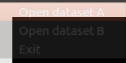
\includegraphics[height=2.0cm,width=6.0cm]{img/cap5/openFile.png}}
\hspace{0.5cm}
%\subfigure[]{\label{fig:LG_hombot}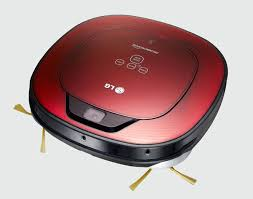
\includegraphics[height=6.0cm]{img/cap2/LG_hombot.jpg}}
\end{center}
%\caption{Robot Dyson 360 Eye (a) Robot Roomba 966 (b) Robot Hombot de LG (c).}
\caption{Selección de archivos de entrada }
\end{figure}

Con el ratón podremos girar en 3 dimensiones  la nube de puntos, acercarnos a el (Zoom in) o alejarnos (Zoom Out),
tambien permite leer un segundo conjunto de puntos 3D y estimar las transformaciones ( rotaciones , traslaciones, escala etc)  necesarias para pasar desde el conjunto de datos ground truth hasta este segundo conjunto de datos. El conjunto de datos resultante tras aplicar las estimaciones será visulalizado en pantalla como otra nube de puntos 3D

Esta herramienta poseé varios modulos accesibles desde el interfaz gráfico. Entre estos módulos podríamos destacar el \textbf{Módulo Transformador}.
Este módulo permite realizar transformaciones sobre el conjunto de puntos 3D groundTruth, de tal forma que se obtendrá como resultado una segunda nube de puntos transformados.
Los parámetros del módulo transformador serán accesible por pantalla
Entre las transformaciones permiten hacer cambios en :
\begin{itemize}
\item ESCALA
\item TRASLACIONES en ejes X,Y,Z
\item ROTACIONES en ejes X,Y,Z
\item Offset de tiempo
\item Interpolación
\item Ruido gaussiano
\item Ruido Cósmico
\end{itemize}

\begin{figure}[H]
\begin{center}
\subfigure[]{\label{fig:transformaciones}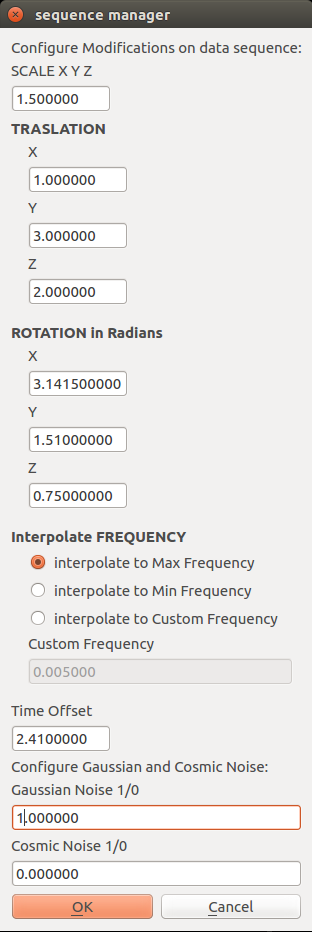
\includegraphics[height=12.0cm,width=4.0cm]{img/cap5/imgTransformaciones.png}}
\hspace{0.5cm}
%\subfigure[]{\label{fig:LG_hombot}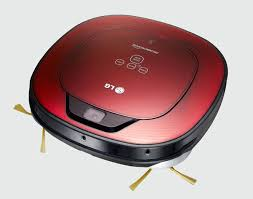
\includegraphics[height=6.0cm]{img/cap2/LG_hombot.jpg}}
\end{center}
%\caption{Robot Dyson 360 Eye (a) Robot Roomba 966 (b) Robot Hombot de LG (c).}
\caption{Detalle de la ventana de configuración de los parámetros de transformación }
\end{figure}


El formato del conjunto de datos ground-truth será timestamp, posición x, posición y, posición z, q0, q1 ,q2 ,q3 . Donde q0,q1,q2,q3 definen un quaternio.
A continuación un ejemplo de los datos de entrada:
\begin{figure}[H]
\begin{center}
\subfigure[]{\label{fig:data example}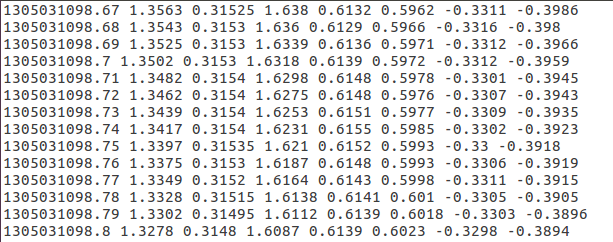
\includegraphics[height=3.0cm,width=8.0cm]{img/cap5/dataExample.png}}
\hspace{0.5cm}
%\subfigure[]{\label{fig:LG_hombot}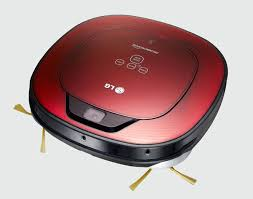
\includegraphics[height=6.0cm]{img/cap2/LG_hombot.jpg}}
\end{center}
%\caption{Robot Dyson 360 Eye (a) Robot Roomba 966 (b) Robot Hombot de LG (c).}
\caption{Ejemplo de los valores de los campo de cada registro del fichero de entrada. }
\end{figure}


Posteriormente tras aplicar las transformaciones definidas en el interfaz gráfico sobre el ground truth, la herramienta devolverá los resultados de estimar dichas transformaciones.


A continuación describiremos en detalle las transformaciones permitidas por la herramienta

\textbf{Escala}. Permite modificar los datos de entrada a nivel de escala. La escala siempre será mayor que cero y se admitirán números con reales

\textbf{Traslaciones}. Se podrán definir traslaciones sobre cada uno de los 3 ejes de coordenadas. 
La traslación admite números reales positivos y negativos.

\textbf{Rotaciones}. Se podrán definir rotaciones sobre cada unos de los 3 ejes de coordenadas. El valor de cada rotación se insertará en Radianes. Los valores admitidos serán números reales tanto positivos como negativos

\textbf{Offset de tiempo}. Con el offset de tiempo podremos introducir un gap en los valores de timestamp del fichero de entrada que más tarde podremos estimar. La exactitud del offset será de centésimas, es decir con 2 decimales

\textbf{Interpolación}: Se podrán realizar 3 tipos de interpolación de los datos.
	Interpolación a la frecuencia máxima
	Interpolación a la frecuencia mínima
	Interpolación a frecuencia personalizada

\textbf{Ruido Gaussiano}: Una de las transformaciones que podremos aplicar sobre el conjunto de datos del groundtrouth es aplicar un ruido gaussiano a los datos transformados

\textbf{Ruido Cósmico}: Otra transformación a aplicar sobre los datos transformados es la incorporación del ruido cósmico

\textbf{Menu de estimaciones}:


Una vez hemos aplicado las transformaciones sobre el groundtrouh, se generará como resultado un nuevo dataset, el transformado.
El menú gráfico nos permitirá estimar que transformaciones se han realizado, y se podrán estimar en 2 sentidos de aplicación, para ello deberemos utilizar el textbf{Módulo Estimador} accesible desde la barra de menú de SLAMTestBed

\begin{figure}[H]
\begin{center}
\subfigure[]{\label{fig:menu A to B y B to A}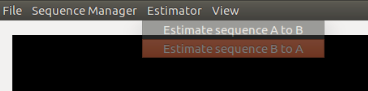
\includegraphics[height=3.0cm,width=8.0cm]{img/cap5/menuAtoB_BtoA.png}}
\hspace{0.5cm}
\end{center}
\caption{Transformaciones permitidas sobre el dataset de entrada }
\end{figure}
	Desde el groundtrouth estimar que transformaciones se han aplicado para llegar a la secuencia de datos transformados. ( A To B)

	Desde la secuencia transformada estimar las transformaciónes para obtener el groundtrouth . ( B to A)
Estas 2 estimaciones se han realizado aplicando cálculos matemáticos tipo SVD y PCA sobre las matrices de datos.
Tambien existe la posiblidad de realizar estas estimaciones transformaciónes utilizando el algortimo RANSAC
Al terminar de calcular las estimaciones aparecerá una ventana con los resultados de las estimaciones calculadas
\begin{figure}[H]
\begin{center}
\subfigure[]{\label{fig:Transformaciones versus Estimaciones}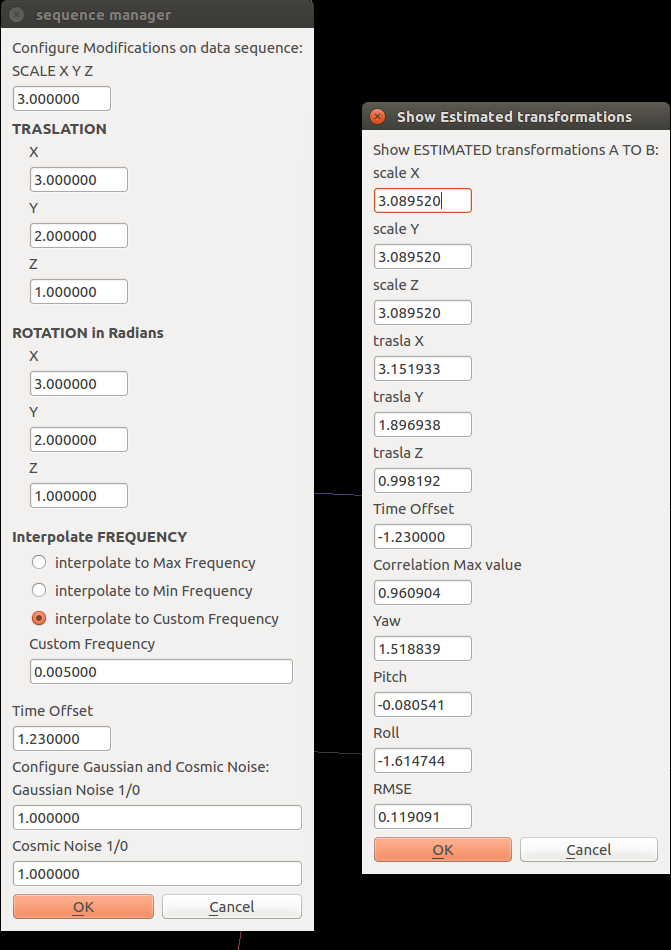
\includegraphics[height=12.0cm,width=8.0cm]{img/cap5/showTransformationsEstimated.png}}
\hspace{0.5cm}
\end{center}
\caption{Transformaciones realizadas frente Transformaciones estimadas }
\end{figure}


\begin{figure}[H]
\begin{center}
\subfigure[]{\label{fig:menu A to B RANSAC}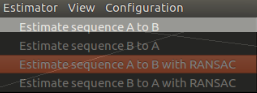
\includegraphics[height=3.0cm,width=8.0cm]{img/cap5/menuEstimatorRANSAC.png}}
\hspace{0.5cm}
%\subfigure[]{\label{fig:LG_hombot}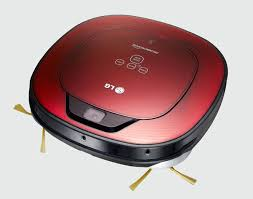
\includegraphics[height=6.0cm]{img/cap2/LG_hombot.jpg}}
\end{center}
%\caption{Robot Dyson 360 Eye (a) Robot Roomba 966 (b) Robot Hombot de LG (c).}
\caption{Transformaciones permitidas con RANSAC sobre el dataset de entrada }
\end{figure}


\textbf{Otras particularidades del menú gráfico}:
La barra de menu de SLAMTestbed, tambien tiene el elemento \textbf{View}. Este elemento de menu ofrece varias opciones gráficas a aplicar sobre los puntos 3D de los conjuntos, y estas son:
\begin{figure}[H]
\begin{center}
\subfigure[]{\label{fig:opciones de View}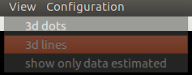
\includegraphics[height=3.0cm,width=8.0cm]{img/cap5/dotsAndLines.png}}
\hspace{0.5cm}
%\subfigure[]{\label{fig:LG_hombot}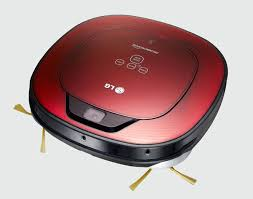
\includegraphics[height=6.0cm]{img/cap2/LG_hombot.jpg}}
\end{center}
%\caption{Robot Dyson 360 Eye (a) Robot Roomba 966 (b) Robot Hombot de LG (c).}
\caption{Transformaciones permitidas con RANSAC sobre el dataset de entrada }
\end{figure}
\textbf{Unir con lineas todos los puntos de cada dataset}. Esta opción es especialmente util cuando estemos utilizando ruido cósmico, ya que al unir los puntos con líneas podremos ver con claridad los puntos con elevado nivel de ruido, que deberían ser tratados como outliers.

\begin{figure}[H]
\begin{center}
\subfigure[]{\label{fig:opciones de View}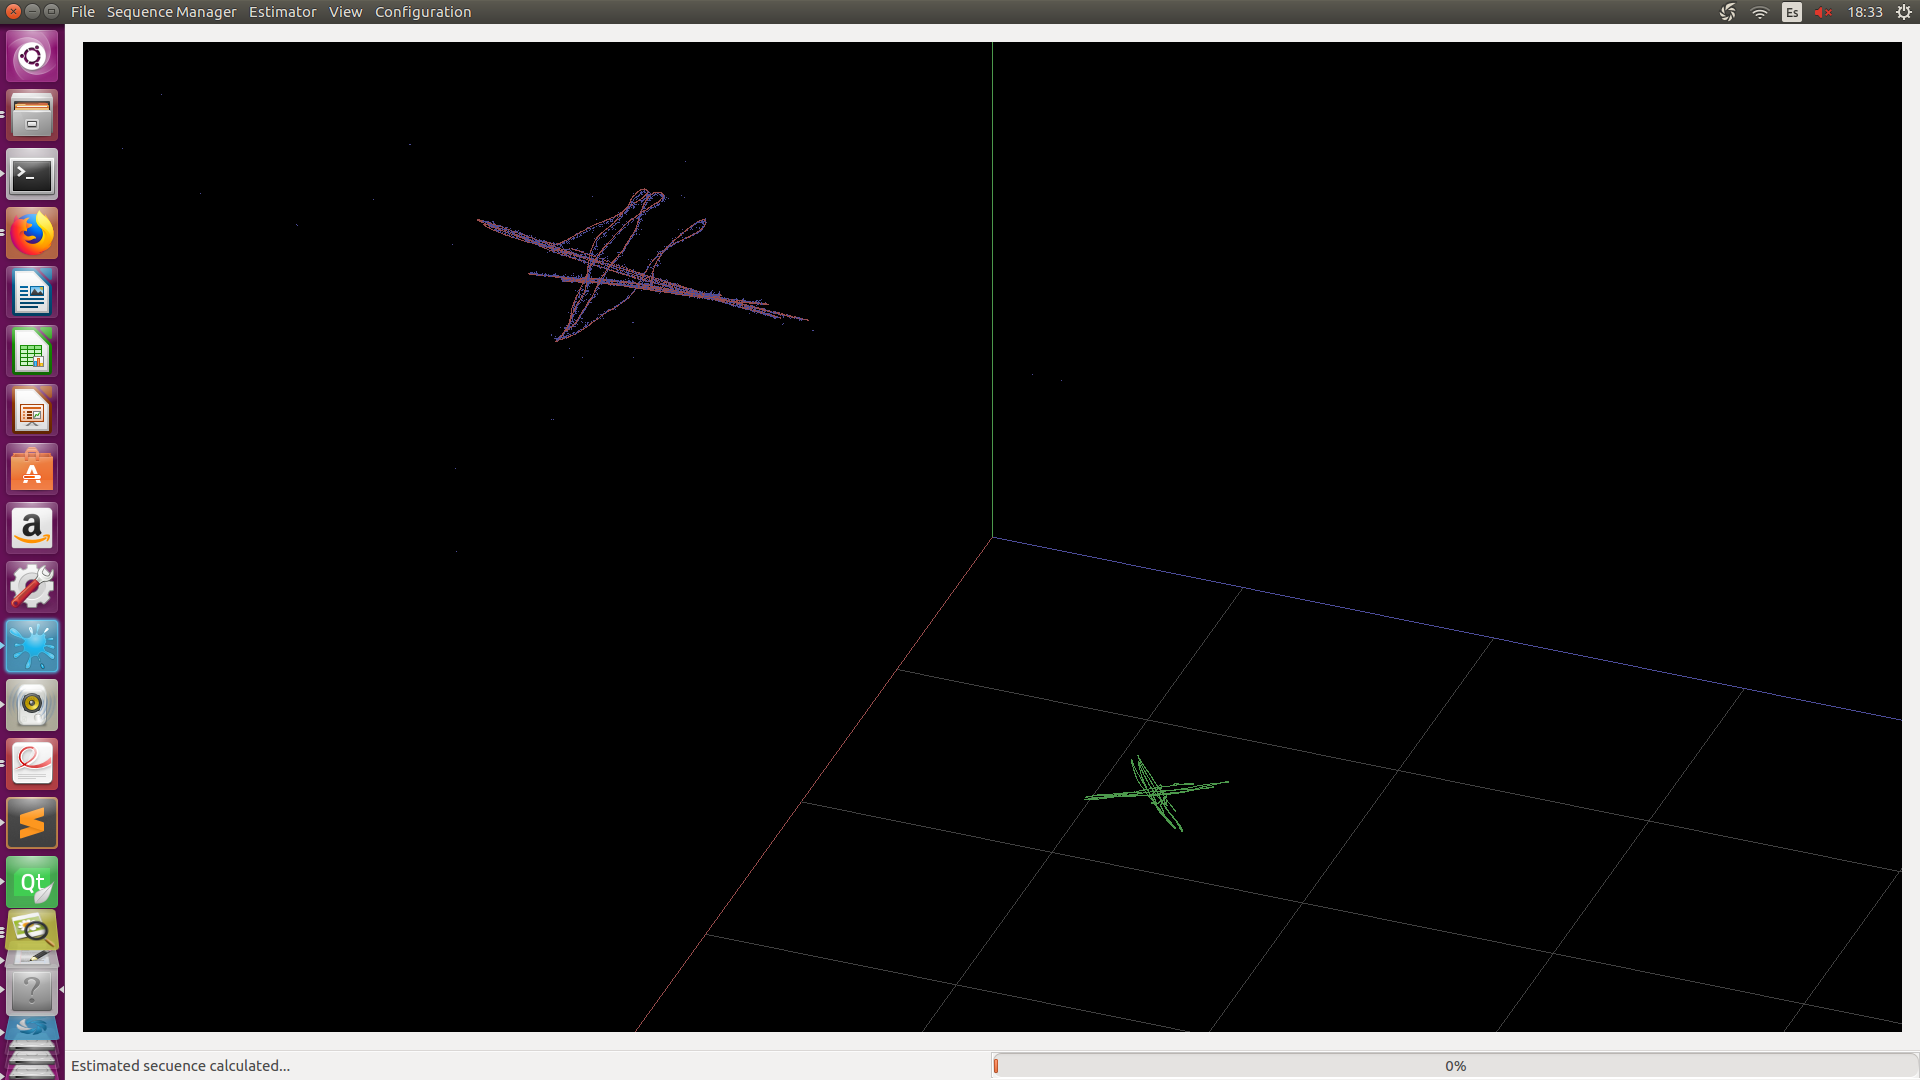
\includegraphics[height=5.0cm,width=10.0cm]{img/cap5/3dDots.png}}
\hspace{0.5cm}

\end{center}

\caption{Ejemplo de datasets visualizados como puntos 3D. Los puntos con ruido cósmico apenas se aprecian. }
\end{figure}


\begin{figure}[H]
\begin{center}
\subfigure[]{\label{fig:opciones de View}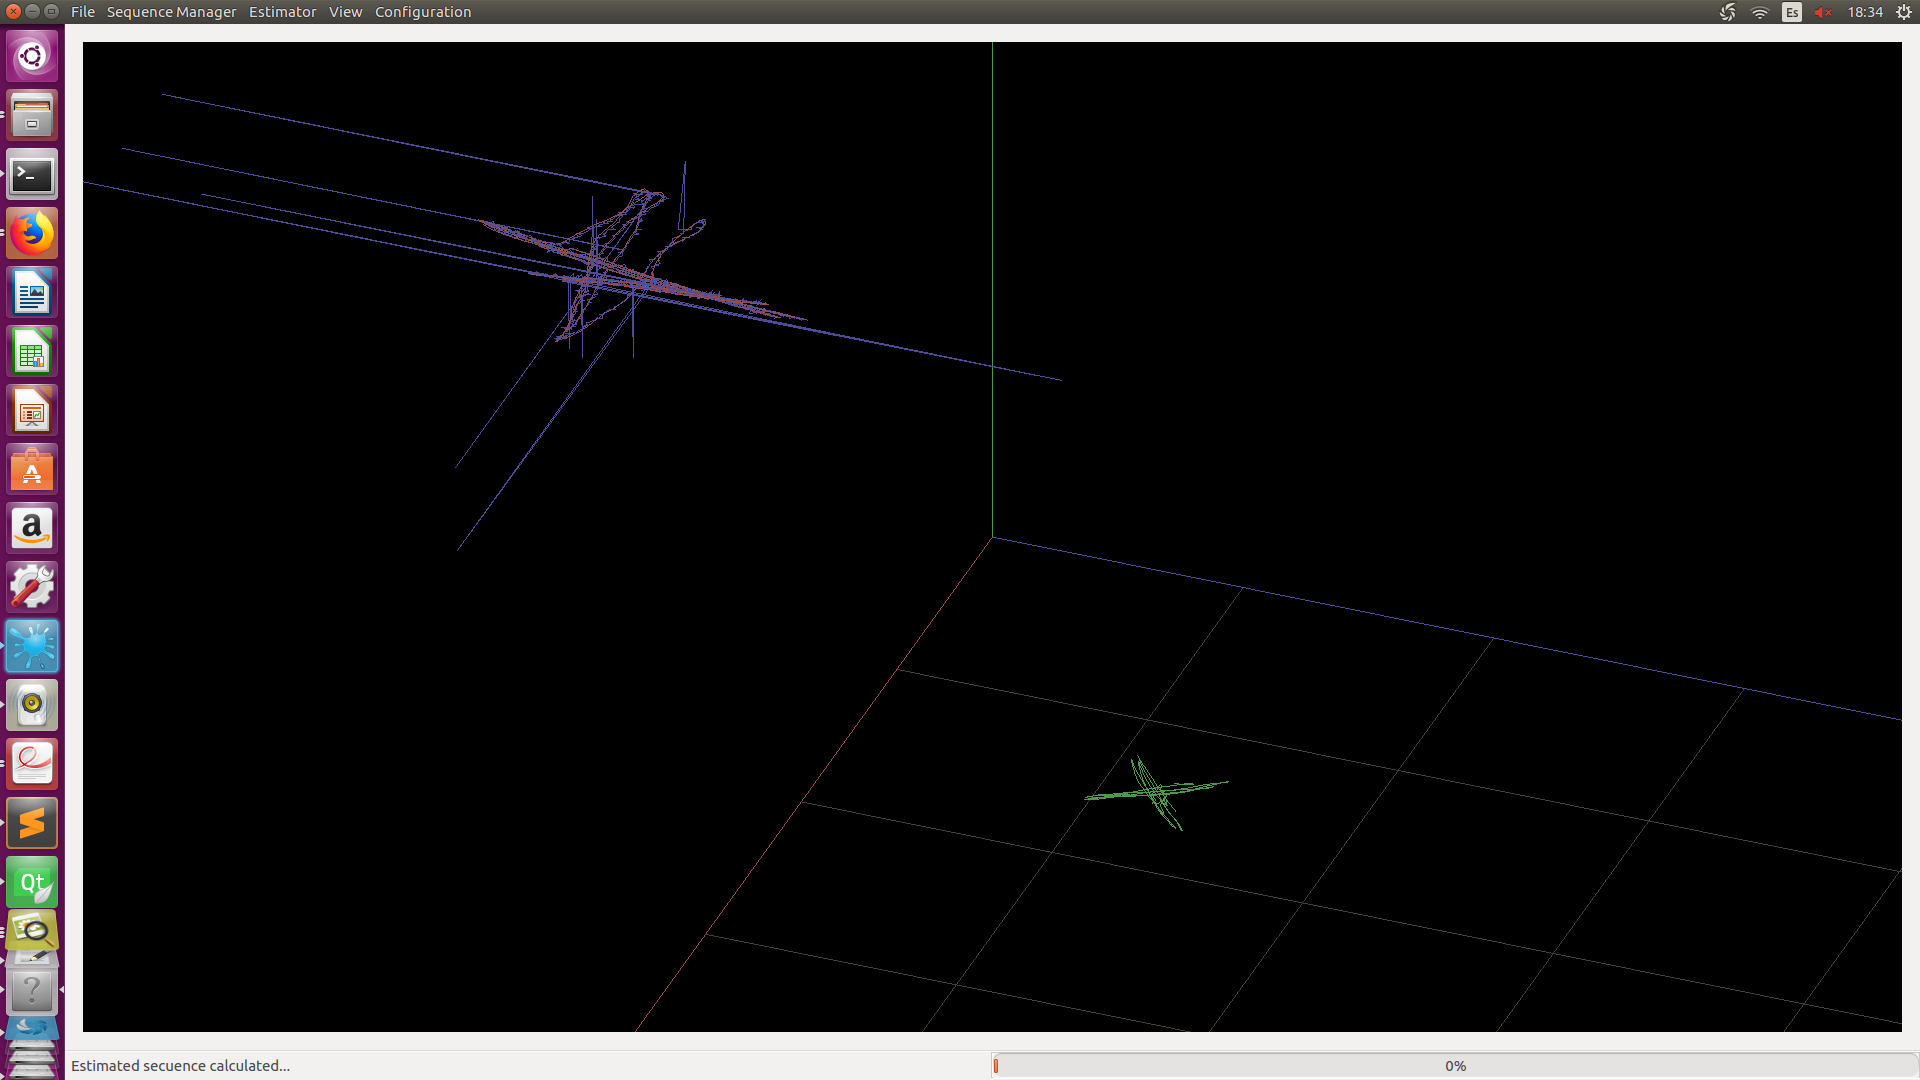
\includegraphics[height=5.0cm,width=10.0cm]{img/cap5/3dLines.png}}
\hspace{0.5cm}

\end{center}

\caption{Ejemplo de datasets visualizados como líneas 3D donde se aprecian mejor los puntos con ruido cósmico}
\end{figure}

Las opciones del menú View tambien permiten sólo visualizar los puntos 3D resultado de las transformaciones estimadas.

    
    

